\SourcePage{GELFAND-P000454}{unlabelled}
\uuline{D. Kazhdan}.\quad Tate's art., Matematika, \underline{$13:2$, §$3$}.

(on the field $\mathbb C_p$ — completion of the alg. closure $\overline{\mathbb Q}_p$ or
$\mathbb Q_p$ — $p$-adic numbers)
\Unclear{GELFAND-P000454}{q-p-link-word}{The connecting word reads “or.”}
\end{GelfandAdjacentEvidence}
\begin{GelfandAdjacentEvidence}{GELFAND-P000454}{2}


\begin{center}
\rule[.5ex]{14mm}{.35pt}\enspace$\cdot$\enspace\rule[.5ex]{21mm}{.35pt}
\end{center}

$K$ — finite ext. of the field $\mathbb Q_p$.

\SourceFigure{GELFAND-P000454}{vertical-ring}{There is a curved stroke between the two entries. Its meaning is uncertain. Two short vertical strokes sit below the second entry.
\par\smallskip\centering\color{black}
\begingroup\color{black}\GelfandFitDiagram{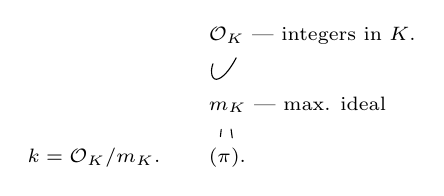
\begin{tikzpicture}[x=1mm,y=1mm,line cap=round,every node/.style={inner sep=0pt,anchor=base west,font=\scriptsize}]
\node at (0,1) {$k=\mathcal O_K/m_K$.};
\node at (23,16.5) {$\mathcal O_K$ — integers in $K$.};
\draw (23.6,13.6) .. controls (23.2,12.55) and (23.45,11.3) .. (24.35,11.7)
  .. controls (25.15,12.05) and (25.95,13.2) .. (26.55,14.35);
\node at (23,7.7) {$m_K$ — max. ideal};
\draw (24.65,5.25)--(24.55,4.35) (25.9,5.3)--(26.05,4.2);
\node at (23,1) {$(\pi)$.};
\end{tikzpicture}}\endgroup}
\end{GelfandAdjacentEvidence}
\begin{GelfandAdjacentEvidence}{GELFAND-P000454}{3}


$L$ — finite ext. of $K$, \sout{\ldots} $\mathcal O_L$ — integers in it

\Unclear{GELFAND-P000454}{ol-cancel}{The crossed-out marks before $\mathcal O_L$ are illegible.}
\end{GelfandAdjacentEvidence}
\begin{GelfandAdjacentEvidence}{GELFAND-P000454}{4}


$m_L=(\tau)$,\quad $\ell=\mathcal O_L/m_L$,
\[
G=\operatorname{Gal}(L:K)
\]
Introduce a filtration in $G$ and prove that $G$ is solvable.

On $L$ and $K$ \sout{\ldots} define a norm so that
$|\pi|=(\operatorname{Card}k)^{-1}$
\Unclear{GELFAND-P000454}{norm-cancel}{A crossed-out sign sits between $K$ and “define.” Its reading is uncertain.}
\end{GelfandAdjacentEvidence}
\begin{GelfandAdjacentEvidence}{GELFAND-P000454}{5}


\uuline{Def.}\quad \sout{\ldots}.
\Incomplete{GELFAND-P000454}{def-cancel}{A short entry is crossed out after “Def.” Its reading is uncertain.}

\[
g\in G_i\Longleftrightarrow \forall x\in \mathcal O_L\quad x^g-x\in m_L^i
\]
\[
G=G_0\supset G_1\supset\ldots\supset G_n=\{e\}.
\]
\end{GelfandAdjacentEvidence}
\begin{GelfandAdjacentEvidence}{GELFAND-P000454}{6}
$G_i$ — normal subgroup in $G$.

\underline{Theorem:}\quad $G_i/G_{i+1}$ — ab. group

$1)$ \underline{$i=0$.}\qquad
$G\overset{\varphi}{\longrightarrow}\operatorname{Gal}(\ell:k)$
(natural map)

\underline{Construction of $\varphi$:}\quad $\bar x\in\ell,\ g\in G$
\[
x\in L\qquad \bar x^g\overset{\mathrm{def}}{=}\overline{x^g}
\]
\Unclear{GELFAND-P000454}{residue-representative}{The manuscript reads $x\in L$.}
\end{GelfandAdjacentEvidence}
\begin{GelfandAdjacentEvidence}{GELFAND-P000454}{7}


$g\in\ker\varphi\Longleftrightarrow \bar x\in\ell,\ \bar x^g=\bar x$,
i.e. $\bar x^g-\bar x=0$, i.e.
\Unclear{GELFAND-P000454}{kernel-quantifier}{The equivalence sign is followed by $\bar x\in\ell$. No explicit quantifier is visible.}
\end{GelfandAdjacentEvidence}



\Needspace{7\baselineskip}
\begin{GelfandAdjacentEvidence}{GELFAND-P000455}{1}
